\documentclass[12pt, a4]{article}
\usepackage[english]{babel}
\usepackage[utf8x]{inputenc}
\usepackage{fullpage}
\usepackage{listings}
\usepackage{graphicx}
\usepackage{color}

%Syntax highlighting
\definecolor{blue-violet}{rgb}{0.54, 0.17, 0.89}
\definecolor{ao}{rgb}{0.0, 0.5, 0.0}
\definecolor{amaranth}{rgb}{0.9, 0.17, 0.31}
\definecolor{ballblue}{rgb}{0.13, 0.67, 0.8}
\definecolor{onyx}{rgb}{0.06, 0.06, 0.06}


\lstset{
  breaklines=true,                 % automatic line breaking only at whitespace
  captionpos=b,                    % sets the caption-position to bottom
  breakatwhitespace=false,
  keepspaces=true,
  numbers=left,
  numbersep=5pt,
  showspaces=false,
  showstringspaces=false,
  showtabs=false,
  tabsize=4,  
  backgroundcolor=\color{white},   % choose the background color
  commentstyle=\color{ao},    % comment style
  keywordstyle=\color{amaranth},    % keyword style
  stringstyle=\color{blue-violet},    % string literal style
  numberstyle=\tiny\color{ballblue},	   % number style
  basicstyle=\ttfamily\footnotesize\color{onyx} % size of fonts used for the code
}

%Document Header
\title{\textbf{Department of CSE\\SSN College of Engineering}}
\author{\textbf{Vishakan Subramanian - 18 5001 196 - Semester VI}}
\date{14 April 2021}

\begin{document}
\maketitle
\hrule
\section*{\center{UCS 1602 - Compiler Design}}
\hrule
\bigskip

%Assignment Details
\subsection*{\center{\textbf{Exercise 7: Generation of Intermediate Code Using Lex and Yacc}}}
\subsection*{\flushleft{Aim:}}
\begin{flushleft}
The new Language Pascal-2021 is introduced with the following programming constructs:\\
\textbf{Datatypes}
\begin{itemize}
\item Integer
\item Real
\item Char
\end{itemize}

\textbf{Declaration Statement}
\begin{itemize}
\item var: type;
\item var: type = constant;
\end{itemize}

\textbf{Conditional Statement}
\begin{itemize}
\item if condition then ----- else ----- endif
\end{itemize}

Generate Intermediate code in the form of Three Address Code sequence for the sample input program written using declaration, conditional and assignment statements in new language Pascal-2021.

\end{flushleft}

%Code
\newpage
\subsection*{\flushleft{Code - Yacc Parser File:}}
\begin{flushleft}
\lstinputlisting[language = C]{TAC.y}
\end{flushleft}

%Code
\newpage
\subsection*{\flushleft{Code - Lex Grammar File:}}
\begin{flushleft}
\lstinputlisting[language = C]{TAC.l}
\end{flushleft}

%Code
\newpage
\subsection*{\flushleft{Sample - Parsed Pascal-2021 Code:}}
\begin{flushleft}
\lstinputlisting[]{Code.txt}
\end{flushleft}

%Output
\newpage
\subsection*{\flushleft{Output 1 - Compilation \& Code:}}
\begin{figure}[h]
\centering
\caption{Console Output - Compilation \& Code.}
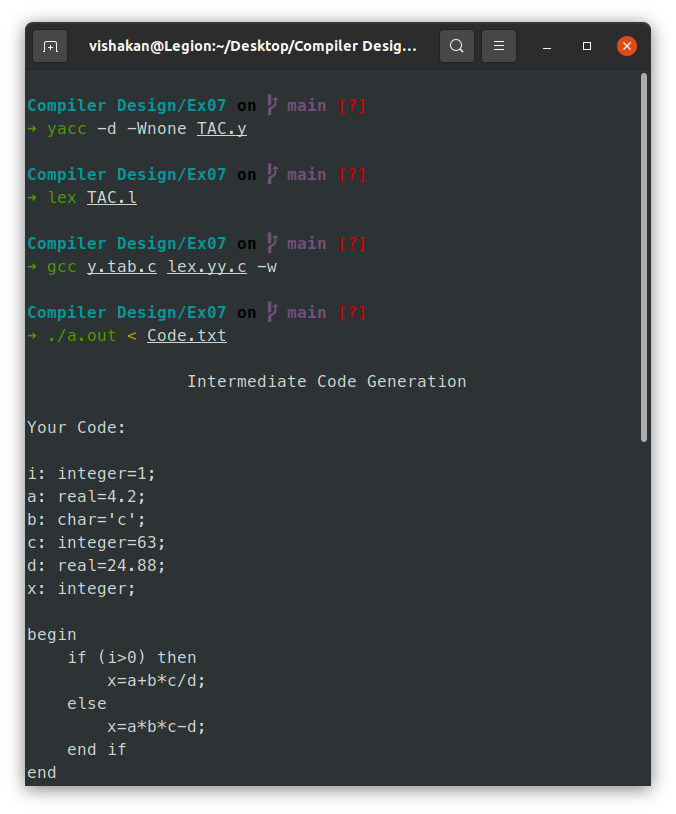
\includegraphics[height=15cm, width=15cm]{Output1.png}
\end{figure}

%Output
\newpage
\subsection*{\flushleft{Output 2 - Intermediate Code:}}
\begin{figure}[h]
\centering
\caption{Console Output - Intermediate Code.}
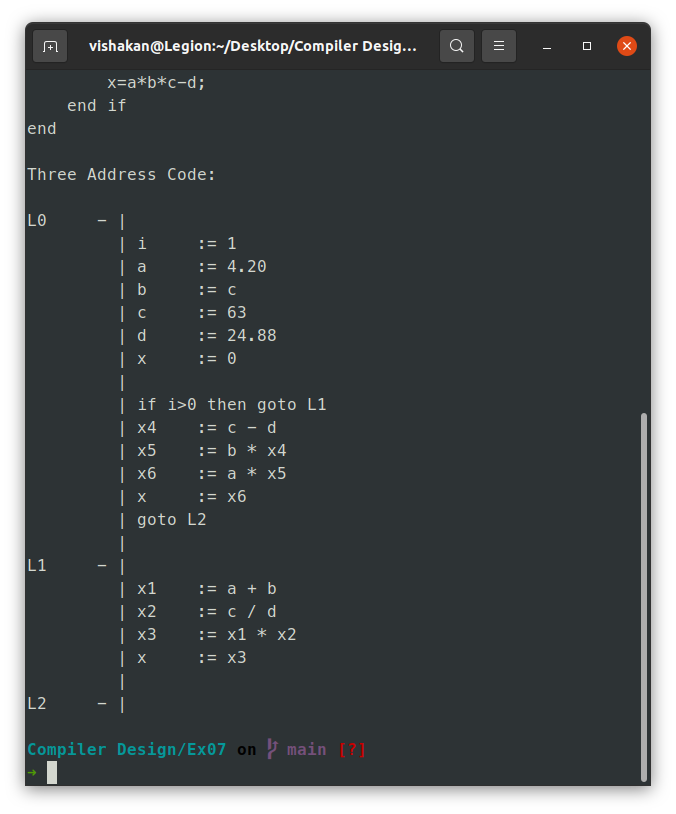
\includegraphics[height=15cm, width=15cm]{Output2.png}
\end{figure}

%Learning Outcome
\newpage
\subsection*{\flushleft{Learning Outcome:}}
\begin{itemize}
\item I learnt more theory behind \textbf{Yacc Parser Generator}.
\item I understood how to construct a grammar for a basic syntax checker.
\item I learnt that grammar can be built upon layer by layer, each one adding more detail and complexity.
\item I was able to implement the required token recognition with Lex tool.
\item I was able to implement the required intermediate code generator with the Yacc tool and Lex tool.
\item I understood the use of the \%union declaration for \textbf{yylval}'s types for passing different values from Lex to Yacc.
\item I declared a custom structure to store intermediate code and variables/values and assigned them values while parsing the respective grammar using the \$\$ operator of Yacc.
\item I made use of the \textbf{sprintf()} function to create intermediate code conveniently.
\item I understood that precedences can only be given to tokens in Yacc, and not for grammar symbols.
\item I was able to construct intermediate code for conditional block with appropriate grammar definition.
\item I came to know that there was no need to return the structures I created inside the parsing of a lower grammar to pass it up to the higher grammar, as it gets implicitly passed up and can be called with the \$ operator.
\item I understood that subtle grammar differences need to be made in the Yacc grammar definition to work for right and left associativity \& precedences.
\item I learnt to call yyerror() with a custom error message within the Lex code.

\end{itemize}


\end{document}
